\section{Data curation}
\label{sec:data}
The main outcome is weekly national DF cases from the Ministry of Health Weekly
Infectious Disease Bulletin on data.gov.sg, 2012--2022 (574 epi weeks)
\citep{mohbulletin}. Dengue
haemorrhagic fever (DHF) is retained separately but not modelled because it averages
less than one case per week. We use NEA/Meteorological Service Singapore (MSS) daily
rainfall and temperature at Changi station S24, aggregated to Monday--Sunday weeks.
Weekly relative humidity comes from the Open-Meteo archive because MSS daily files do
not include humidity \citep{mssdaily,openmeteo}. The brief's MOH 2014--2018 file is an
independent source check and secondary analysis \citep{mohbrief}.

MOH epi weeks follow the MMWR Sunday--Saturday calendar (2014 and 2020 have week 53).
Each week is keyed by the following Monday to align with weather. The bulletin and the
2014--2018 file agree exactly on 209 of 261 overlapping DF weeks; the maximum weekly
difference is 8 cases and totals differ by about 0.2\%. The largest DHF difference is
one case. There are no duplicate or missing case weeks. Weather quality checks found no
implausible values. MSS and Open-Meteo weekly temperature correlate at $r=0.91$ (Open-Meteo
is 1.3$^\circ$C cooler); rainfall correlation is $r=0.48$. Open-Meteo humidity correlates
with NEA monthly Changi humidity at $r=0.56$ and is 5.8 percentage points higher on average.

Cases are aggregated national notifications, not individual records; no personal
information is used. Weather and cases are joined by \texttt{week\_start}, with weather lags
calculated before joining. Source links, licences, retrieval manifest, variable definitions,
inclusion rules and further QA results are documented in \texttt{docs/DATA.md}. These
data choices limit interpretation: one station may not represent local rainfall, and
reported cases reflect testing and reporting as well as transmission.

\begin{figure}[ht]
  \centering
  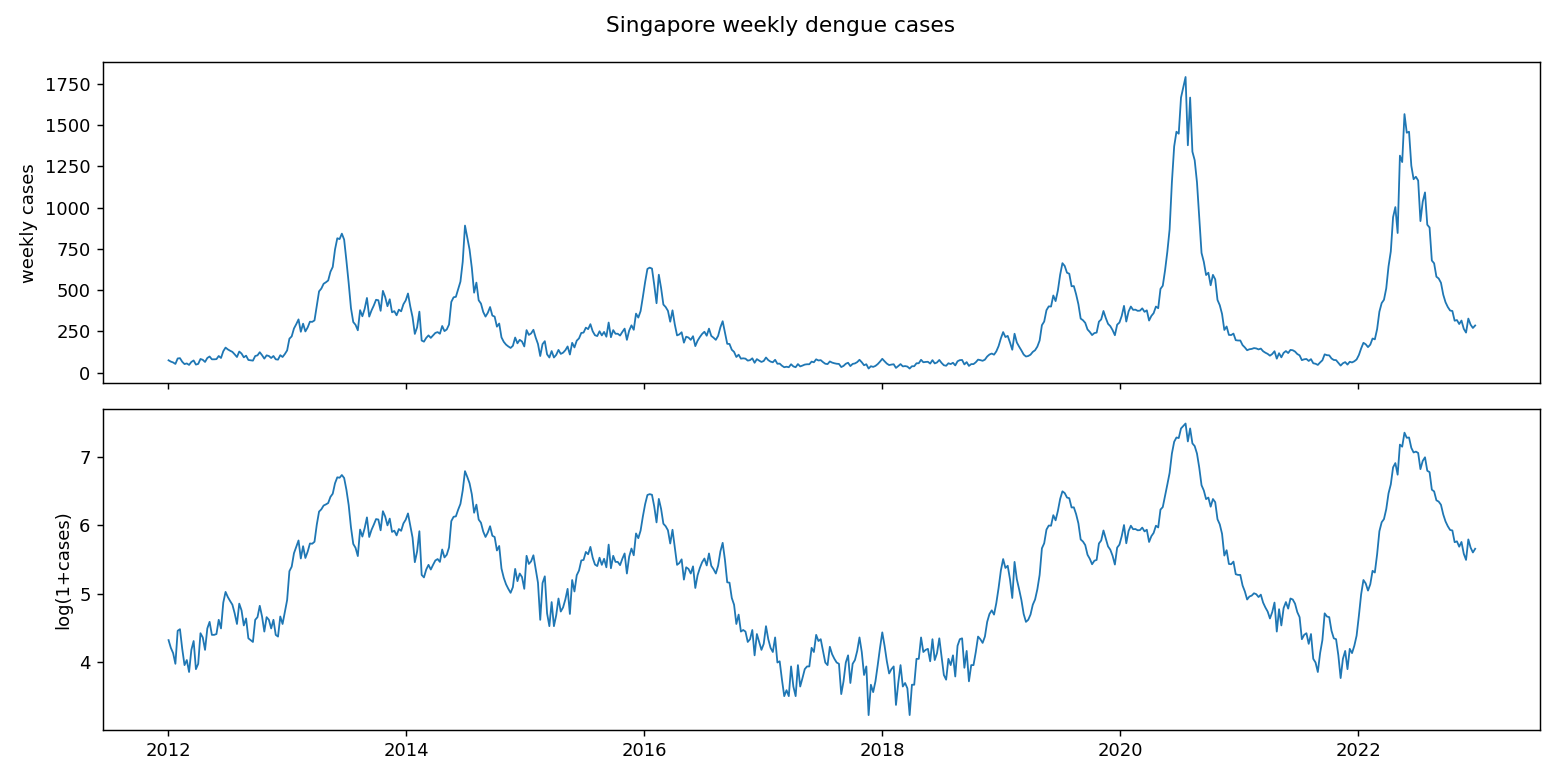
\includegraphics[width=0.9\linewidth]{eda_cases_timeseries.png}
  \caption{Weekly dengue fever counts in the main series; DHF is not included in the target.}
  \label{fig:cases}
\end{figure}
